\chapter{Protokolle}
	\section{Regensensor CON-REGME-24V}
		Im Datenblatt wurde bezüglich des Regensensors CON-REGME-24V eine maximalen Stromaufnahme von 230 mA angegeben. Als der Regensensor in Betrieb genommen wurde fiel auf, dass er mehr als angeben benötigt. Aus diesem Grund wurde eine Messreihe diesbezüglich aufgenommen und einen Grund für das Verhalten zu ermitteln.
		
		\begin{table}[H]
			\centering
			\begin{tabular}{|l|l|l|}
				\hline \textbf{Max Ampere} & \textbf{Erster Testlauf} & \textbf{Zweiter Testlauf}\\
				\hline 1,5A& 10ms & 5ms\\
				\hline 1,0A& 10ms & 10ms\\ 
				\hline 0,75A& 15ms & 14ms\\ 
				\hline 0,5A& 25ms & 27ms\\ 
				\hline 0,3A& 57ms & 53ms\\ 
				\hline 0,3A& nicht ermittelbar & nicht ermittelbar\\
				\hline
			\end{tabular}
			\caption{Abbauzeiten bzgl. der Strombegrenzung des Regensensors}
			\label{table:RainmA}
		\end{table}
		
		In der Tabelle \ref{table:RainmA} wird dargestellt, wie lang die Stromversorgung in die Strombegrenzung geht, sobald der Strom eingeschaltet wird. Der Effekt tritt allerdings nur auf, wenn man den Sensor in Verbindung mit der eingebauten Heizung verwendet.
		
		Es kann nur vermutet werden, das die ermittelten Werte auf den Kaltleitereffekt der Heizung zurückzuführen sind. Dieser Effekt gibt an, das der Widerstand des Leiters im kalten Zustand relativ gering ist und sich bei Erwärmung deutlich erhöht. Somit würde über den Leiter, bis er sich erwärmt hat, ein hoher Strom fließen.
		
		In den folgenden Abbildungen sieht man die genauen Oszilloskop-Messergebnisse.
		
		\begin{figure}[H]
		\centering
		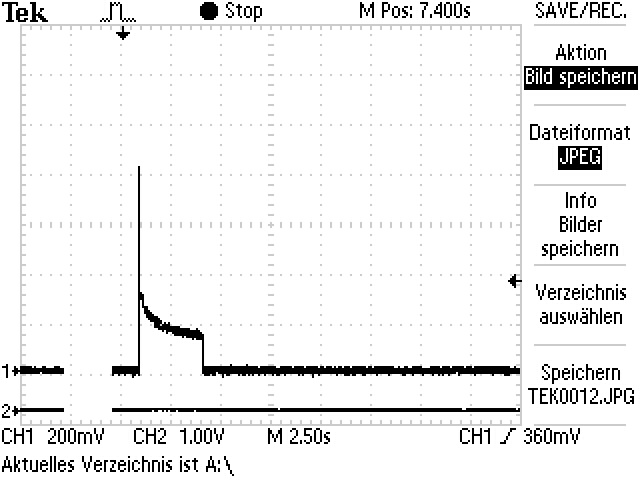
\includegraphics[width=10cm,height=5cm]{./Grafiken/TEK0012}
		\caption{Messung bei einer Strombegrenzung von 1,5A}
		\label{fig:TEK0012}
		\end{figure}
		
		\begin{figure}[H]
		\centering
		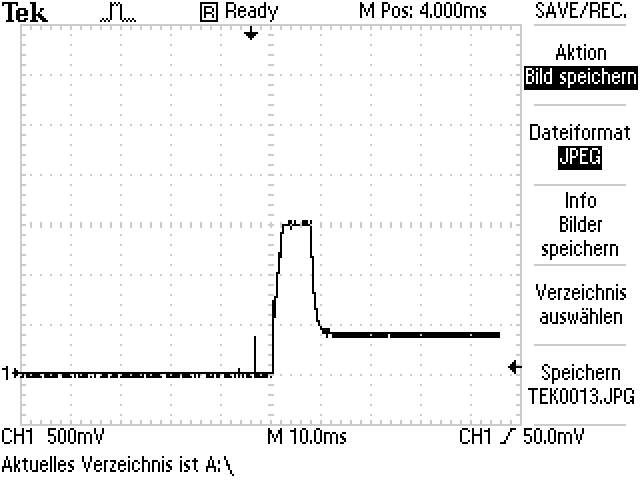
\includegraphics[width=10cm,height=5cm]{./Grafiken/TEK0013}
		\caption{Messung bei einer Strombegrenzung von 0,5A}
		\label{fig:TEK0013}
		\end{figure}
		
		\begin{figure}[H]
		\centering
		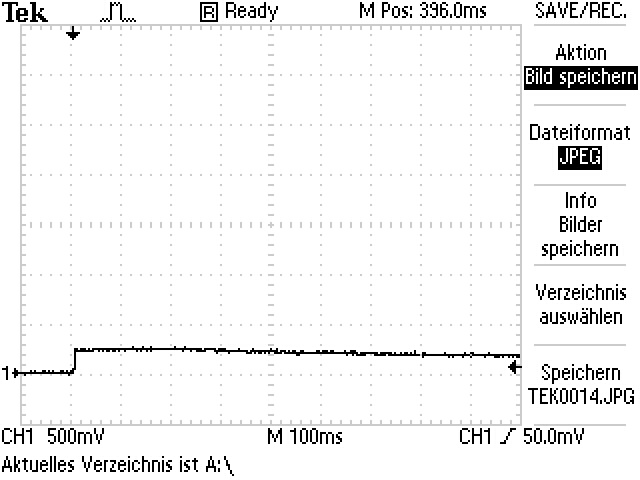
\includegraphics[width=10cm,height=5cm]{./Grafiken/TEK0014}
		\caption{Messung bei einer Strombegrenzung von 0,23A}
		\label{fig:TEK0014}
		\end{figure}
		
		In der letzten Abbildung \ref{fig:TEK0014} war der Unterschied zwischen Strombegrenzung und Leistungsaufnahme so gering, dass kein Zeitpunkt bestimmt werden konnte, ab dem die Heizung auf Betriebstemperatur ist. Deswegen kann in der Tabelle \ref{table:RainmA} kein Wert angegeben werden.
		
		Als Resultat muss der Sensor, sofern er mit der integrierten Heizung verwendet wird, über eine separate Spannungsversorgung betrieben werden. Wäre dies nicht der Fall, so würde ein Spannungszusammenbruch die gesamte restliche gekoppelte Elektronik beeinflussen. Alternativ muss extra für diesen Sensor eine Strombegrenzung eingesetzt werden, die die Spannung in der Restschaltung konstant hält.
	\section{Feuchte-/Temperatur Sensoren HYT271/241}
		Um bezüglich dieser Sensoren eine Aussage über die Genauigkeit geben zu können, wurde eine Reihe von Messungen durchgeführt. Um einen Referenzwert bezüglich der gelieferten Sensordaten geben zu können wurden zwei weitere Geräte verwendet. Einerseits das Klimalogg Pro\footnote{Etwa 100\euro{}} und andererseits das Medbus\footnote{Etwa 10\euro{}}.
		
		Da die Messungen allerdings nur exemplarisch durchgeführt wurden und dies nicht in einer Klimakammer mit speziellen Messbedingungen erfolgte, kann mit den folgenden Ergebnissen keine exakte Aussage getroffen werden. Es kann lediglich grob abgeschätzt werden, ob die Sensoren bezüglich der Referenzgeräte exakt arbeiten.
		\subsubsection{Messergebnisse bezüglich der relativen Luftfeuchtigkeit}
		
		\begin{table}[H]
			\centering
			\begin{tabular}{|l|l|l|l|l|}
				\hline \textbf{Ort der Messung} & \textbf{HYT271} & \textbf{HYT241} & \textbf{Medbus} & \textbf{Klimalogg Pro}\\
				\hline Arbeitszimmer & 45,2 & 46,1 & 51 & 52 \\
				\hline Balkon & 53,5 & 55,0 & 49 & 60 \\
				\hline Kühlschrank & 59,3 & 62,8 & 50 & 53 \\
				\hline Schrank & 57,2 & 58,1 & 49 & 49 \\
				\hline Badezimmer & 68,5 & 71,7 & 55 & 65 \\
				\hline 
			\end{tabular}
			\caption{Messergebnisse bezüglich der relativen Luftfeuchtigkeit (in \%)}
			\label{table:HYTHumid}
		\end{table}
		
		Man kann anhand den Daten sehen, das die Messwerte der Sensoren in der selben Größenordnung der Referenzgeräte liegen. Es sind allerdings auch deutliche Abweichung zu erkennen. Ohne Tests in einer Klimakammer kann hierzu allerdings keine weitere Aussage getroffen werden.
		
		\subsubsection{Messergebnisse bezüglich der Temperatur}
		
		\begin{table}[H]
			\centering
			\begin{tabular}{|l|l|l|l|l|}
				\hline \textbf{Ort der Messung} & \textbf{HYT271} & \textbf{HYT241} & \textbf{Medbus} & \textbf{Klimalogg Pro}\\
				\hline Arbeitszimmer & 20,6 & 20,8 & 19,5 & 19,7 \\
				\hline Balkon & 5,7 & 6,1 & 7,2 & 5,7 \\
				\hline Kühlschrank & 8,4 & 8,5 & 9,1 & 9,5 \\
				\hline Schrank & 17,0 & 17,6 & 19,1 & 19,1 \\
				\hline Badezimmer & 19,7 & 20,3 & 19,8 & 20,6 \\
				\hline
			\end{tabular}
			\caption{Messergebnisse bezüglich der Temperatur(in °C)}
			\label{table:HYTTemp}
		\end{table}
		
		Bezüglich der Temperatur passen die Messergebnisse deutlich besser als bei der relativen Luftfeuchte. Jedoch ist auch hier eine sehr große Abweichung zu erkennen. Es gilt ebenfalls, das ohne Tests in einer Klimakammer keine weiteren Aussagen getroffen werden können.